\chapter{POVQAD数据集构建}\label{dataset}
CLEVR数据集与积木世界具有极高的相似度,在积木世界相关的人工智能研究领域具有重要应用。
然而CLEVR存在存在场景完全可见、不要求模型使用外部背景知识进行推理等不足之处,无法满足本文
“提升神经符号方法在部分可见积木世界场景下的空间推理问答的准确率”的总目标。
本章旨在构建积木世界部分可见空间推理数据集,以便在后续研究中评估本文提出的神经符号VQA框架的性能,为本文的总研究目标服务。
下面分别就构建目标、构建原则、构建流程及统计与合理性分析方面展开介绍。
\section{构建目标}
本文在第一章中指出,本文研究的总目标是提升神经符号方法在部分可见积木世界场景下的空间推理问答的准确率,
并且在第二章对CLEVR数据集进行介绍时指出,尽管CLEVR数据集与积木世界具有极高的相似度,
但存在场景完全可见、不要求模型使用外部背景知识进行推理、封闭式唯一解的不足,难以作为评估模型在部分可见积木世界场景中空间推理能力的有效基准。
基于本文的总研究目标和CLEVR数据集的不足,本文提出构建一个积木世界部分可见场景空间推理数据集(Partial Observation VQA Dataset, POVQAD)
,以便在后续的研究中评估本文提出的神经符号VQA框架的性能。

从具体方面而言,POVQAD数据集的构建目标主要包括以下几个方面:
\begin{enumerate}[itemsep=0pt,parsep=0pt]
\item \textbf{图像组成}:本文借鉴CLEVR数据集的设计方案,在图像包含的物体的属性上,设置了
形状、尺寸、材质和颜色四种属性。尺寸的可能取值为小、中、大;颜色的可能取值为红色、蓝色、绿色、黄色、灰色、棕色、紫色和青色;
材质的可能取值为橡胶和金属;形状的可能取值为圆锥体、球体、圆柱体和立方体。选取这四种基本属性,
是因为它们是物体最直观且容易区分的特征,并且与原始 CLEVR 数据集保持一致,便于进行比较研究。对每个属性的可能取值
进行了限制(例如,八种颜色,四种形状,两种材质,三种尺寸),这样做的目的是为了简化
推理过程并控制答案的搜索空间,避免由于可能的属性组合过多而导致的推理复杂度过高。

对图像空间的划分,采用四分区域设定的方案,其取值为 0、1、2、3。由于所有图像都被划分成
4个区域,故图像中物体也会处在某一个区域之中。为了研究问题方便,本文规定每个物体只能在图像的一个区域中,不能
同时跨多个区域。为图像空间划分区域,主要的优势在于
为图像生成和问题生成指定作用范围约束,有利于提升数据集的复杂性和多样性。
约束指的是对物体的属性组合、物体之间的关系、物体在空间中的位置等进行限制的一组规则。
在POVQAD中,从作用范围来看,约束可以分为区域约束、跨区域约束和全局约束。
区域约束是仅作用于特定区域的局部规则。例如,“区域1中所有物体形状必须为立方体”。
跨区域约束是涉及多个区域的全局规则。例如,“区域1和区域2中同颜色物体的总数不超过2个”。
全局约束是适用于整个场景的通用规则。例如,“所有物体必须属于至少一个区域”或“不允许存在完全相同的两个物体属性组合”。

在生成问题、图像时,可以通过使用约束来施加限制条件,例如“区域1中的不能有球体”,在空间区域与物体属性之间建立了联系
,进而生成更加多样化的问题和图像,提升数据集的复杂性和多样性。
此外,生成的问题中,一方面可以考察满足指定特征的物体所在的区域,另一方面问题也可能会要求模型在解答其它问题时考虑物体所在的
区域,进而考察模型在空间推理中的能力。

约束通过使用ASP来进行表示。例如:
\begin{lstlisting}
    :- obj(X), at(X, 0), not has_property(X, shape, cube), not has_property(X, shape, cylinder).
\end{lstlisting}
表示如果X在区域0,那么它的形状必须是立方体或圆柱体。
\item \textbf{问题类型}:在原始的CLEVR数据集中,包括属性查询、计数、比较属性、比较数量和存在性问题
一共五类问题,在POVQAD数据集中,删除了是否类问题(即比较属性、比较数量和存在性问题)以及计数问题,仅保留属性查询类问题。
采取该方案基于以下几点考量:(1)POVQAD的核心目标是评估模型在部分可见积木世界场景中对目标物体属性的推理能力,尤其强调
在只有一部分信息和环境约束之下,通过排除法找出符合条件的物体的可能属性值;
(2)是非题和计数问题通常返回的是一个布尔值或者整数,不需要明确识别不可见物体的属性。ASP求解器在解决此类问题时,
整个求解过程往往不具备复杂的排除性与可解释性;
(3)属性查询类问题的问题目标是询问不可见物体的某个属性是什么,ASP求解器对该类问题的求解过程可以形成明显的逻辑链条,
从部分信息及环境约束中推导出不可见物体的属性值;
因此,属性查询类问题更加契合“通过环境约束与部分观测信息联合推导目标物体属性”的这一目标,本文在POVQAD
中仅保留属性查询类问题。

根据属性查询类问题的目标以及图像可能包含的物体属性,问题可划分为尺寸、材质、颜色、形状、区域共计5类属性查询问题。
\item \textbf{答案组成}:
\end{enumerate}

基于上述构建目标,本文将POVQAD数据集形式化定义为一个五元组的集合:
$$D = \{ (I_i,P_i,Q_i,\Pi_i ,A_i) | i=1,2,...,N \}$$
其中,每个元素$(I_i,P_i,Q_i,\Pi_i ,A_i)$是数据集中的一个样例,各组成部分定义如下:
\begin{enumerate}[itemsep=0pt,parsep=0pt]
\item \textbf{$I_i$}为图像,是通过 Blender 渲染的基于 ASP 场景图生成的 3D 图像。
每张图像表示一个三维积木世界场景,所有可见物体均按预定义属性摆放。每个图像中都刻意隐藏了一个物体,以模拟部分可见条件。
\item \textbf{$S_i$}为场景,是对当前图像中所有可见物体的ASP表示,采用ASP进行表示。
其中主要包含以下内容:每个可见物体的属性,包括尺寸、颜色、材质、形状;每个物体所属的区域;可见物体之间的空间关系,如\textbf{left(X,Y)}表示X在Y的左边;
被隐藏的物体(即问题中提及而图像中不存在的物体)不会出现在部分场景信息中。
\item \textbf{$Q_i$}为问题,使用自然语言形式进行表示,例如“What shape is the small red object that is to the left of the yellow cube?”。
所有问题均为属性查询类问题,专门针对物体的四个属性之一:颜色、尺寸、形状或材质。
\item \textbf{$QA_i$}为问题的ASP表示,例如:
\begin{lstlisting}
query(Q) :-
    has_property(X, color, Q),
    has_property(X, shape, cylinder),
    has_property(Y, shape, sphere),
    has_property(Y, color, red),
    left(Y, X),
    same_material(X, Y),
    X != Y.
\end{lstlisting}
\item \textbf{$\Pi_i$}为环境,是当前图像所属环境的一组约束规则,采用ASP进行表示。以下为一组约束示例:
\begin{lstlisting}
% 约束示例
% 区域0中所有物体的形状必须是圆柱体
:- obj(X), at(X, 0), has_property(X, shape, cylinder).
% 区域1中蓝色物体的数量大于2个
:- #count{X: has_property(X, color, blue), at(X, 1)} > 2.
\end{lstlisting}
\item \textbf{$A_i$}为答案集,
\end{enumerate}

POVQAD数据集采用 ASP 作为统一的表示与推理语言,贯穿于环境约束的定义、完整场景图的生成与问题的形式化表示
三个核心环节。具体原因如下:
\begin{enumerate}[itemsep=0pt,parsep=0pt]
\item ASP支持高层次知识建模。POVQAD所涉及的空间推理任务,本质上是一个多层次的知识表示与约束求解问题。
环境约束定义了某类场景中物体属性分布的全局或局部规则;场景图构建要求从这些规则中生成满足逻辑一致性的物体布局;
问题表示与求解则需要基于观察到的部分信息,反推出隐藏物体的属性。
在这些任务中,ASP具有以下核心优势:(1)声明式建模,使用逻辑规则直接描述“应该满足什么”,
而不是“如何计算”,避免编程过程的冗余细节;(2)非单一模型求解,ASP可自动求解所有满足条件的模型,天然适合多解推理任务;
(3)支持不完备信息建模,通过否定与缺省推理机制,可以有效表示部分可见性下的场景;
(4)可组合性强,环境约束、已知信息与问题查询均可通过逻辑程序合并输入,实现统一推理。
\item 在环境约束生成中,ASP能够高效表达复杂的属性限制。环境约束可能包括限制属性取值(如“区域0中所有物体必须是红色或黄色”)、
限制物体数量(如“区域1中恰好有2个小物体”)、跨区域比较(如“区域1和区域2中相同颜色的物体数不能超过3”)以及
排他性限制(如“不得存在两个属性完全一致的物体”)。这些约束结构灵活,复杂度高,传统的数据生成方法难以精确表达。而 ASP 的规则语法(例如 :- 引入约束,\#进行计数等)非常适合表达此类逻辑条件。
\item 在场景图构建中,ASP可有效保障逻辑一致性。在场景图构建过程中,ASP求解器被用作生成器,即在给定环境约束的前提下,
通过ASP求解器获得符合约束的场景图。每个完整场景图对应一组ASP事实;ASP求解器在物体属性组合与区域位置上
进行求解;最终仅保留满足所有约束条件的合法解集,用于渲染与问题生成。通过在场景图构建中使用ASP求解器,
可以系统性地采样出大规模、逻辑一致、属性多样的积木世界场景,避免人工构造或启发式方法中可能出现的歧义与逻辑错误。
\item 在问题表示中,ASP实现了可求解性与可解释性的统一。POVQAD中的问题不仅以自然语言形式存在,
还被转换为对应的ASP查询规则,这一方案的优势包括:(1)问题可直接嵌入ASP推理流程,与部分场景信息与环境约束统一求解;
(2)保证所有问题均具有可求解性:Clingo 求解器可验证其是否有合法答案;(3)通过分析解集大小、排除路径等,可进行问题难度分级与推理链可视化;
(4)每个问题的“答案空间”明确,适用于多解式评估与开放性回答。

例如,问题“与红色球体右侧的物体具有相同材质的物体的颜色是什么?”可形式化为:
\begin{lstlisting}
query(Q) :-
    has_property(X, color, Q),
    has_property(X, shape, cylinder),
    has_property(Y, shape, sphere),
    has_property(Y, color, red),
    right(Y, X),
    same_material(X, Y),
    X != Y.
\end{lstlisting}

这种形式使得问题的语义清晰、结构明确,便于执行与验证。
\end{enumerate}

\section{构建原则}
本节要给出具体构建方法,含技术和实现;

本文旨在构建一个部分可见积木世界场景的空间推理VQA数据集(POVQAD),用以模拟
现实世界中信息缺失的场景,并评估模型的空间推理能力。为实现该目标,本文在POVQAD数据集的构建中
遵循如下原则:
\begin{enumerate}[itemsep=0pt,parsep=0pt]
\item \textbf{部分可见性}:每个样本场景中有一个目标物体被隐藏,
图像和逻辑表示中均不可见,以此模拟现实中因遮挡或感知局限导致的信息缺失情境。
\item \textbf{逻辑一致性}:每个场景都必须满足由 ASP 定义的一组环境约束,
保证场景内部在逻辑层面上的合理性,避免不同约束之间发生冲突。例如,不能同时出现“区域1中所有物体都是蓝色”和“区域1中没有蓝色的物体”这种自相矛盾的约束。
\item \textbf{显式知识整合}:问题的求解不仅依赖图像中可见的感知信息,
还必须结合背景约束与已知事实进行逻辑推理,从而考察神经符号系统的知识整合能力。
\item \textbf{可追溯性与可解释性}:每一条样本数据均包含场景图、问题、背景知识,
可由 Clingo 求解器还原推理过程,便于可解释性研究。
\end{enumerate}
\section{构建流程}
POVQAD的构建流程如图\ref{}所示,

\subsection{环境生成}
在POVQAD中,一个环境是一个由一组约束规则组成的逻辑框架,用于限定在该环境下生成的所有场景所必须满足的
属性组合、区域位置等先验知识。在数学上可以集合来表示环境:
$$\varepsilon = \{ C_1, C_2, ..., C_k \}, C_i \in ASP \quad Constraint$$
其中,每个$C_i$是用ASP表示的一条逻辑约束规则。

环境的生成过程包括以下步骤:(1)预定义11种约束模板;(2)每个环境实例随机选取并实例化
最多15条约束模板;(3)确保每个环境中至少包括区域级约束和跨区域约束;(4)对所有生成的约束经语义检查与逻辑一致性
验证。

约束模板的设计参考了POVQAD中的物体属性值设定,此外也参考了
Visual Abductive Reasoning\cite{liang2022visualabductivereasoning}中引入区域/跨区域推理的设计思路,
以及Neurosymbolic Reasoning Benchmarks\cite{bortolotti2024neurosymbolicbenchmarksuiteconcept}中
用于ASP场景建模的约束形式。

本文规定POVQAD的每个环境最多由15条约束规则模板实例化构成,这一数值是经过多方面权衡确定的,目的主要在于以下几方面:
\begin{enumerate}[itemsep=0pt,parsep=0pt]
\item 逻辑复杂度与可解性的平衡。如果某个环境中的约束规则过少,会导致后续生成的场景图过于松散,
物体属性组合高度自由,推理空间过大,导致问题复杂度过大,难以进行有效推理。
如果约束规则过多,则会造成约束之间产生冲突,导致ASP求解器难以知道合法的解,影响求解效率,进而影响场景图的生成。
\item 控制生成时间与可维护性。每条规则在 ASP 中都可能极大影响解空间,规则数上升将显著增加 ASP 求解时间。此外,
在大规模数据生成中,15 条以内的环境可以在数秒内稳定求解出场景图,利于批量生成和调试。
\end{enumerate}

在生成环境的过程中,规定每个环境中至少包括区域级约束和跨区域约束,共计两种约束。做出这一规定的目的在于
增强环境的逻辑层次性与推理深度,具体原因如下:
\begin{enumerate}[itemsep=0pt,parsep=0pt]
\item 支持多层次推理链的构造。区域级约束用于构建局部一致性,跨区域约束用于建模全局对比或协同关系。
同时使用这两类约束,可以使推理问题具有从局部到跨区域的空间层级,增加问题的空间深度。
\item 避免场景构造退化为简单的组合。如果只使用区域级约束,那么后续根据环境生成场景图时,将会变成多个局部区域的简单组合,
缺乏各个区域之间的相互关联。添加跨区域约束之后,有助于生成具有全局一致性/相互限制/相互支撑的复杂场景图。
\item 支撑部分可见场景下的间接推理。在部分场景图中,若不可见物体在区域0中缺失,模型可以通过区域0的其它规则
或者区域0与区域1的对比或者联动规则来进行属性排除或依存判断。而如果采用单一的区域级约束,
那么对于区域0中的物体的问题,模型只能依赖于区域0的局部信息进行推理,缺乏全局视角,不利于考察模型的宏观层面推理能力。
\end{enumerate}

进行语义检查与逻辑一致性验证的具体方案是用ASP求解器(本文中采用Clingo)对生成的约束尝试进行求解,
如果Clingo没有提示错误信息,并且能够成功求解出至少一个合法的解集,则说明该环境的约束规则是逻辑一致的,并且
能够顺利通过语法检查。本步骤的主要目标是避免后续出现死循环、空解等问题。

部分约束模板的ASP编码表示以及对应表示含义见表\ref{tab:asp_templates}。
最终,一共生成了30个环境,数据集中的所有场景图均匀分布在这些不同的环境之中。
环境的具体示例见附录\ref{appendix:environment}。
\begin{table}[h]
    \centering
    \renewcommand{\arraystretch}{1.0}
    \begin{tabular}{|p{3cm}|p{12cm}|}
        \hline
        \textbf{模板} & \textbf{描述} \\
        \hline
        \textbf{模板1(取值约束)} & 
        \texttt{:- obj(X), at(X, R), not has\_property(X, P1, V1).} \\ 
        & 解释: 对区域R中的所有物体,它们P1属性的取值均为V1。 \\ 
        & 具体实现: :- obj(X), at(X, 0), not has\_property(X, color, red). \\
        \hline
        
        \textbf{模板2(否定约束)} & 
        \texttt{:- obj(X), at(X, R), has\_property(X, P1, V1).} \\ 
        & 解释:对区域R中的所有物体,它们的P1属性的取值,均不能为V1。 \\ 
        & 具体实现::- obj(X), at(X, 0), has\_property(X, material, metal). \\
        \hline
        
        \textbf{模板3(恰有N个约束)} & 
        \texttt{:- \#count\{X: has\_property(X, P1, V1), obj(X), at(X, R)\} != N.} \\ 
        & \textbf{解释}:在区域R中,恰好有N个物体的P1属性的取值为V1。 \\ 
        & 具体实现::- \#count\{X: has\_property(X, size, small), obj(X), at(X, R')\} != 2. \\
        \hline
        
        \textbf{模板4(至少有N个约束)} & 
        \texttt{:- \#count\{X1, X2: sameProperty(X1, X2, P1), obj(X1), obj(X2), at(X1, R1), at(X2, R2)\} < N.} \\ 
        & 解释:在区域R1和区域R2中,至少有N对物体,它们的P1属性的取值都是V1。 \\ 
        & 具体实现::- \#count\{X1, X2: sameProperty(X1, X2, shape), obj(X1), obj(X2), at(X1, 1), at(X2, 2)\} < 1. \\
        \hline
        
        \textbf{模板5(或约束)} & 
        \texttt{:- obj(X), at(X, R), not has\_property(X, P1, V1), not has\_property(X, P1, V2).} \\ 
        & 解释:区域 R中的所有对象都具有属性 P1 的 V1 值或属性 P2 的 V2 值。 \\ 
        & 具体实现::- obj(X), at(X, 1), not has\_property(X, color, yellow), not has\_property(X, color, blue). \\
        \hline
    \end{tabular}
    \caption{部分约束模板示例}
    \label{tab:asp_templates}
\end{table}
\subsection{完整场景图构建}
在获得特定环境后,使用 ASP 求解器在逻辑层面构建符合这些约束的完整场景图。
场景图是场景的ASP表示,场景是场景图在图像层面的具体体现。
为了具体说明两者之间的关系,下面通过一个例子予以说明。在某个场景图中,包含以下ASP规则:
\begin{lstlisting}
obj(0). has_property(0, color, red). has_property(0, shape, cube). at(0, 1).
obj(1). has_property(1, color, green). front(1, 0).
\end{lstlisting}
该场景图可以通过Blender渲染为图像场景,该图像中有一个红色立方体出现在区域1中,
同时还有一个绿色的物体出现在该红色立方体的前方。

生成完整场景图的步骤如下:
\begin{enumerate}[itemsep=0pt,parsep=0pt]
\item 设定生成目标。在生成的环境的基础之上,还需要指定当前希望生成的场景图中包含多少个物体,以及物体属性的可选范围。
本文设定场景图中物体数量为4到9,其余四种物体的属性设定按照先前章节中的约定执行:
\begin{lstlisting}
% 颜色可取值范围是红色、蓝色、绿色、黄色
color(red; blue; green; yellow).
% 物体的形状可取值范围是立方体、圆柱体、球体
shape(cube; cylinder; sphere).
% 物体的材质可取值范围是金属、橡胶
material(metal; rubber).
% 物体的尺寸可取值范围是小、大
size(small; large).

obj(0..5). % 生成编号为0到5的物体,总共6个物体。要生成其它数量的物体,只需要修改这里的数字即可。
\end{lstlisting}
\item 编写ASP生成规则。为了给每个物体生成属性,需要编写ASP规则来让ASP求解器为物体分配属性。
\begin{lstlisting}
1 { has_property(X, color, C) : color(C) } 1 :- obj(X).
1 { has_property(X, shape, S) : shape(S) } 1 :- obj(X).
1 { has_property(X, size, Z)  : size(Z)  } 1 :- obj(X).
1 { has_property(X, material, M) : material(M) } 1 :- obj(X).

1 { at(X, 0..3) } 1 :- obj(X).  % 每个物体只能在一个区域中
\end{lstlisting}
通过ASP中的选择规则(choice rules),要求ASP求解器从可能的值中选择一个赋给物体的属性。
\item ASP求解器生成解集。
使用 Clingo 等 ASP 求解器,将“环境 + 属性范围 + 生成规则”作为输入,ASP求解器会搜索满足所有约束的解空间,并输出一组满足条件的回答集。
以下是一个可能的解集示例,构成了一个完整场景图。其中涉及到的谓词的功能如下:谓词\texttt{obj}用于定义不同的物体(所有物体的名称用0,1等数字来表示)。
谓词\texttt{has\_property(obj, Attribute, Value)}用于将对象的名为Attribute的属性的值设置为Value。
对象之间的空间关系用谓词\texttt{left}、\texttt{right}、\texttt{front}、\texttt{behind}来表示,例如
\texttt{left(A, B)}表示B位于A的左侧。
\begin{lstlisting}
%场景中的物体
obj(0). obj(1). obj(2). obj(3).

%物体的属性
at(0, 2).
has_property(0, color, green).
has_property(0, size, large).
has_property(0, material, rubber).
has_property(0, shape, cylinder).
....

%物体间的空间关系
front(1, 0). right(1, 0). ...
\end{lstlisting}
\item 验证与采样。在通常情况下,ASP求解器会为每个环境会生成成千上万条符合条件的回答集。本文采取随机采样
的策略以选取场景图,目的在于以下几点:(1)控制数据集的规模。每个场景图后续要生成图像、问题、ASP表示、答案,
如果不采样,那么数据规模会指数增长,造成资源浪费,并且生成的场景图也需要人工审核,如果场景图规模过大,
将会很难进行有效的审核;(2)确保样本的多样性。ASP求解器会返回多个合法的回答集,但无法保证这些回答集在属性组合上的多样性,
如果不随机采样,而是直接选取前若干条或者后若干条,会导致模式重复。而采用随机采样的方法,可以打乱解集的顺序,
提升物体数量、属性组合分布、不同空间关系分布和场景图在视觉方面的多样性;(3)避免偏差性解集。
在解集空间中,某些满足约束的组合可能更“常见”或“易于求解”,如果直接按顺序采样,会让这些组合比例过高。
随机采样有助于防止数据偏态分布,使模型不会过拟合于高频属性组合。

具体而言,本文使用Python的\texttt{random.shuffle()}将解集进行随机打乱。此后,从每个环境生成的所有场景图中,
采样100个场景图。在采样完成之后,通过人工检查,确保场景图的区域覆盖均衡、属性组合多样并且没有出现重复物体的情况。
\end{enumerate}

最后,在图\ref{pipeline_for_generating_environment}直观展示了从环境到属于该环境的场景图构建的过程。
\begin{figure}
    \centering
    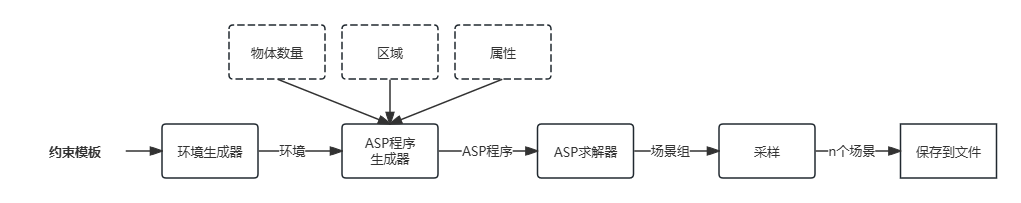
\includegraphics[width=\textwidth]{pipeline_for_generating_environment.png}
    \caption{生成环境以及该环境中的完整场景的流水线}
    \label{pipeline_for_generating_environment}
\end{figure}
\subsection{部分场景图构建}
在构造部分可见场景时,需要从完整场景图中选择一个物体作为被隐藏的目标物体,设为$Obj_i$。
选择目标物体的过程需要满足以下条件:
\begin{enumerate}[itemsep=0pt,parsep=0pt]
\item 从场景图的所有物体中随机选取一个,在随机选取的过程中,要注意保持均衡,不能
一直选取单一区域的物体或者相同属性的物体,以免造成数据偏态分布。
\item 被选择物体不能是唯一出现某一属性的对象,避免由于移除该物体后,
导致场景图中该属性的值无法被推断,导致问题无解。
\item 该物体将在后续问题中作为查询目标。
\end{enumerate}

选择$Obj_i$后,需要将完整场景图中关于$Obj_i$的所有事实全部移除,生成部分场景图。具体需要做到以下几点:
\begin{enumerate}[itemsep=0pt,parsep=0pt]
\item 删除\texttt{obj(i)}、\texttt{at(i, R)}、\texttt{has\_property(i, P, V)};
\item 删除所有涉及$Obj_i$的空间关系谓词,如\texttt{left(i, j)}、\texttt{right(i, j)}等;
\item 保留其余物体的信息与关系。
\end{enumerate}
从而得到一个只包含可见物体的子结构,记为 $Partial_i$,该场景中缺少了目标物体的显式信息。
\subsection{问题生成与逻辑编码}
问题生成与逻辑编码的目标是,围绕每个部分可见场景图构造有意义的查询问题,获得其自然语言描述,并将其转换为ASP查询。
每一个生成的问题,应该满足如下条件:(1)针对被遮挡物体(隐藏对象)的某一属性;
(2)基于剩余可见物体和环境约束进行间接推理;(3)问题语义必须明确且答案集非空。

POVQAD中仅包含属性查询问题,不包括是非题和计数题。查询的属性包括颜色、形状、尺寸和材质。
为了便于控制问题类型的数量分布,本文规定每个问题只能查询上述四个属性中的一个,具体属性由随机策略决定。
考虑到不同种类属性的可能取值数量不同,进而不同属性的问题的可能答案数量也不同,
本文据此规定每种属性的问题在数据集中所占的比例:颜色与形状各占40\%,材质与尺寸各占10\%。

POVQAD采用问题模板来构造自然语言问题,
一种供参考的模板如\ref{asp:question-template}中所示,
其中<Z2>、<C2>、<M2> 表示待查询对象的已知属性(例如尺寸、颜色、材质),由随机策略从完整场景图中选取;
<R> 为空间关系(如left、right、front、behind),其取值既满足随机性,又依赖于完整场景中物体间的真实空间分布;
<Z>、<C>、<M>、<S> 则代表参考对象的属性,
对完整场景图中与查询对象具有特定空间关系的候选对象进行筛选之后确定。

这种模板化设计不仅使自然语言问题的结构化描述成为可能,
而且便于后续转换为ASP的形式化表示,从而实现问题求解的自动化。
\begin{lstlisting}[label=asp:question-template]
What shape is the < Z2 > (size) < C2 > (color) < M2 > (material) [that is] 
< R > (relation) the < Z > (size) < C > (color) < M > (material) < S > (shape) ?
\end{lstlisting}

实例化之后,得到的自然语言问题可能为:\texttt{What shape is the small red rubber object that is left of the large green metal cube?}。
获得自然语言问题之后,再使用ASP对其进行表示。对每一个自然语言问题,都是从一个问题模板出发,填充占位符,
然后生成的。所以,自然语言和ASP查询具有一一对应的逻辑结构,可以实现自动转换。

对上述获得的自然语言问题,解析占位符,可以得到:
\begin{enumerate}[itemsep=0pt,parsep=0pt]
\item 被查询对象:size(small)、color(red)、material(rubber)
\item 参考对象:size(large)、color(green)、shape(cube)
\item 空间关系:left(X, Y)
\item 查询属性:shape
\end{enumerate}

随后自动生成ASP查询规则如下所示,其中X是隐藏对象,Y是参考对象,Q是要查询的属性值,has\_property是表示属性的谓词。
\begin{lstlisting}
query(Q) :-
    has_property(X, shape, Q),
    has_property(X, size, small),
    has_property(X, color, red),
    has_property(X, material, rubber),
    has_property(Y, size, large),
    has_property(Y, color, green),
    has_property(Y, shape, cube),
    left(X, Y),
    X != Y.
\end{lstlisting}

\subsection{答案生成与求解}
答案生成与求解环节的核心任务是:
将问题$Q_i$、部分场景$P_i$与环境约束$\Pi_i$被统一输入给Clingo进行求解,生成答案集$A_i$。
求解目标是确定隐藏物体的某一属性在当前部分信息下的所有合理可能值组成的集合,即答案集$A_i$。
具体步骤如下:

首先,将问题$Q_i$、部分场景$P_i$与环境约束$\Pi_i$,这三部分的ASP表示拼接到同一个\texttt{.lp}文件中,
例如:
\begin{lstlisting}
% 1. 场景信息(Partial_i)
obj(0). obj(1).
has_property(0, color, green).
...

% 2. 环境约束(Env_i)
:- obj(X), at(X, 0), not has_property(X, shape, cube).
...

% 3. 查询规则(Program_i)
query(Q) :- has_property(X, color, Q), ..., same_material(X, Y).
\end{lstlisting}

此后,调用Clingo开始进行求解,并从Clingo的输出结果中提取\texttt{query(Q)}的值集合,例如:
\begin{lstlisting}
query(red) query(green) % 说明 red, green 是该问题的所有可能答案值。
\end{lstlisting}

为了保证问题的质量和有效性,本文对生成的答案集采取了一些筛选措施:(1)答案非空。答案集必须满足$|A_i| \geq 1$
,否则表示该问题无解,需要被排除;(2)答案不全。如果答案集等于该属性所有可能取值(例如颜色有8个取值,结果为8个值),说明该问题逻辑约束不足,属于信息缺失型问题,也将被剔除。
因此筛选条件为:
$$1 \leq |A_i| < |\mathcal{A} |$$
其中$\mathcal{A} $是该查询属性的所有取值集合。

最终,答案被编码为一个取值集合,例如某个查询颜色的问题的答案集为\{ red \},某个查询形状的问题的答案集为
\{ cube, sphere \}。
\subsection{图像渲染与样例生成}
图像渲染与样例生成的目的是将场景图转换为3D图像,以提供用于VQA任务的真实图像输入,并将图像与问题、
答案集进行统一组织,形成可供模型训练和推理的完整样例。本文使用Blender进行图像生成,具体流程如下:
\begin{enumerate}[itemsep=0pt,parsep=0pt]
\item 初始化场景。在这一步中,会设置Blender的一系列渲染参数,包括图像宽度、图像高度、渲染引擎、分辨率百分比等等,以及
配置GPU渲染。
\item 添加对象。将对象添加到场景中,并设置材质、颜色、形状等属性以及所在区域。
\item 检查对象可见性。在渲染之前,需要确保所有对象在图像中可见。具体实现方法是,检查每个对象的像素数量,判断是否满足最低要求,低于最低要求则视为该对象不可见。最低像素数的默认值设置为200,
因为生成的图像的默认分辨率为320x320,200个像素大约占据了图像的0.2\%。这一比例在视觉上足够明显,同时
不会因为分辨率限制而导致过多的场景被丢弃。
\item 执行渲染。渲染当前场景,并将文件保存到指定目录。如果在渲染过程中发生异常,将会进行最多三次的重试。
\item 删除对象。将目标物体从场景中删除,得到最终的图像。
\end{enumerate}

在图像生成完成之后,每一条数据样例$D_i$会被组织为一个JSON对象。JSON对象的结构如下:
\begin{lstlisting}
{
    "question_nl": "What color is the small rubber object to the left of the red cube?",
    "image": "partial_scene_0001.png",
    "answer": ["red", "green"],
    "environment": "环境约束具体内容",
    "scene_asp": "场景图的ASP表示",
    "question_asp": "query(Q) :- has_property(X, color, Q), ...",
}
\end{lstlisting}

最后,所有的数据样例的JSON对象会被统一存储在一个JSON文件中。
\subsection{小结}
图\ref{pipeline_for_generating_partial}展示了构建POVQAD数据集的全过程。
该流程通过随机采样,使生成的问题在属性组合和空间关系上呈现多样性;通过对解集规模的判定机制,
有效过滤掉普遍适用或无区分意义的问题,确保每个问题都能够准确反映场景中物体属性的关系;
使用模板化设计和ASP表示为后续数据集扩充与新问题类型的加入提供了灵活性和统一标准。
\begin{figure}[h]
    \centering
    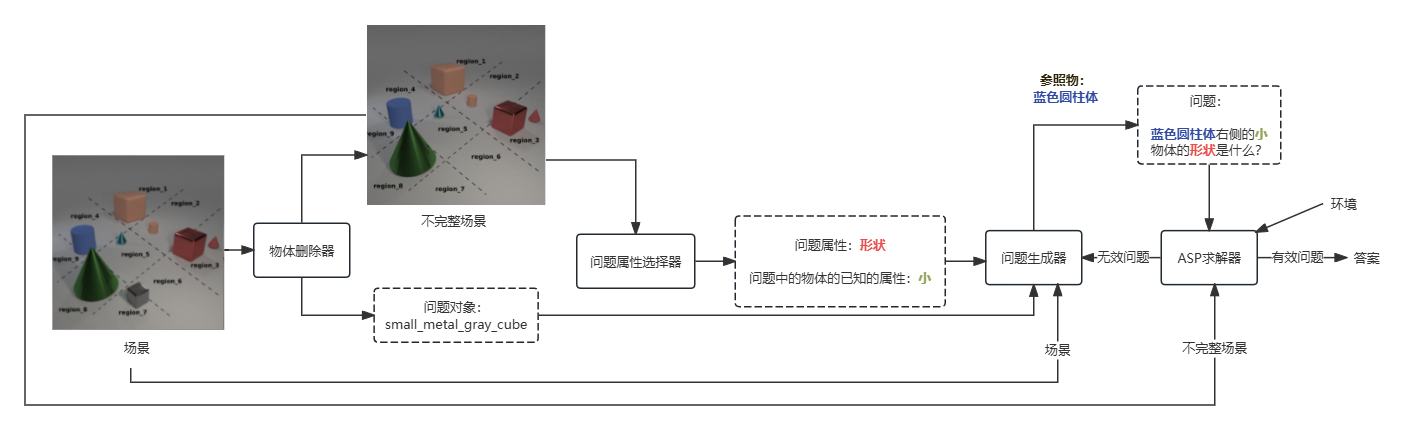
\includegraphics[width=\textwidth]{pipeline_for_generating_partial.png}
    \caption{生成部分场景和问题,并进行标记的流程}
    \label{pipeline_for_generating_partial}
\end{figure}
\section{统计与合理性分析}
\subsection{数据集统计}
问题分布的统计图见图\ref{fig:question_statistics}。从图\ref{fig:question_statistics}(a)中可得知,有关颜色和形状的问题在POVQAD数据集中
占比最高,分别是39\%和37.6\%,关于大小和材质的问题则相对较少,分别只占到了13.6\%和9.8\%。
所提问题的类型取决于被查询的物体的属性,在生成数据集的过程中,允许用户设置问题类型的预期占比。
以上问题类型占比,是基于以下的设置生成的:颜色问题占比40\%,形状问题占比40\%,大小问题占比10\%,材质问题占比10\%。
做出如上设置的原因是,与材质(只有两个值)相比,颜色和形状等属性包含更大的值集合(颜色有 8 个值,形状有 4 个值)。
因此,以颜色为中心的问题的答案集空间比以材质为中心的问题的答案集空间更广,从而为数据集带来了更多样化的答案集空间。

图\ref{fig:question_statistics}(b)、(c)、(d)和(e)分别说明了各种问题类型(尺寸、形状、材质和颜色)的潜在答案的分布。
生成数据集的目标之一是实现均衡的分布,避免大多数问题都导致相同的答案集的情况。
例如,当问题涉及物体的大小时,其可能的解可以是
 \{大, 中\}、\{大, 小\}、\{小, 中\}、\{大\}、\{中\} 或 \{小\} 之一,
 如图\ref{fig:question_statistics}(b)所示。由于查询属性为颜色的问题的可能答案数量很大(因为颜色可以取 8 个值),
 因此图\ref{fig:question_statistics}(e)中并未列出整个空间。根据统计图可以看出,在生成过程中没有偏向任何特定的答案。
\begin{figure}[h]
    \centering
    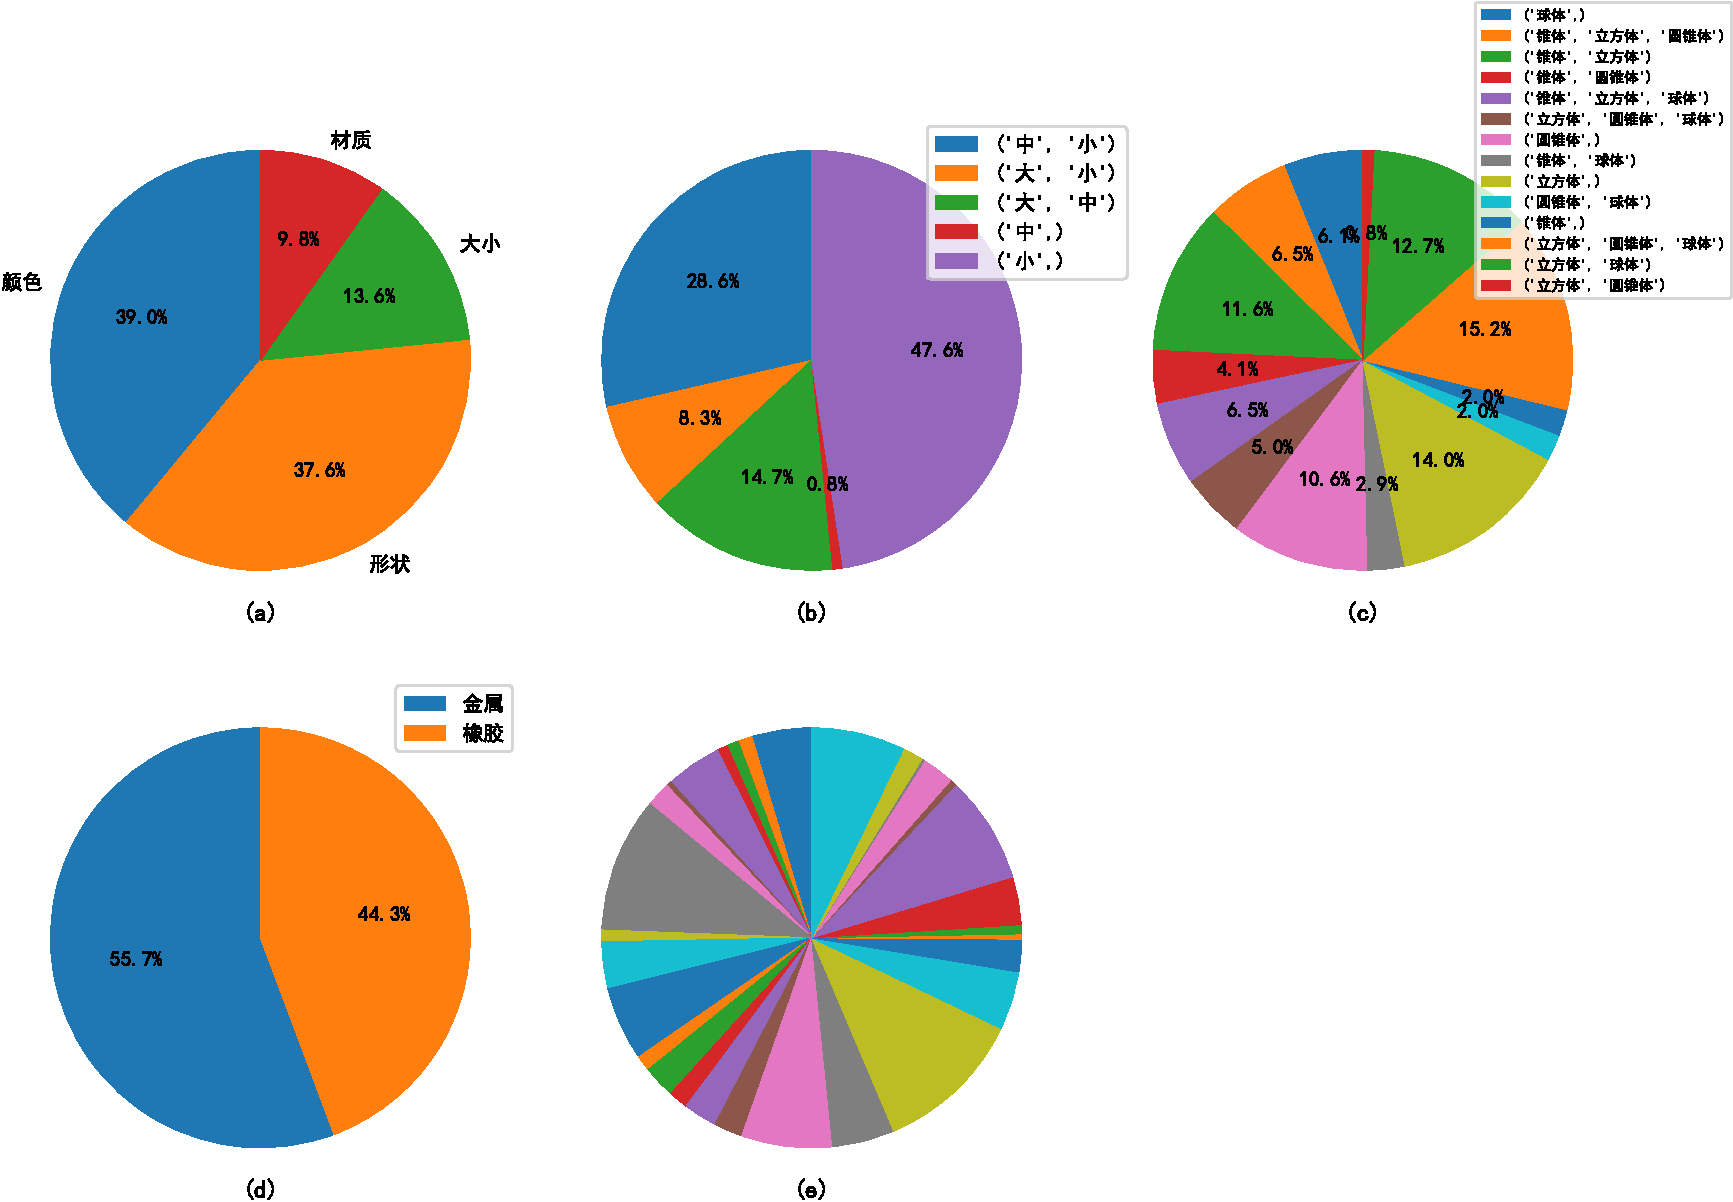
\includegraphics[width=\textwidth]{figures/question_distribution-crop.pdf}
    \caption{问题分布统计}
    \label{fig:question_statistics}
\end{figure}

图\ref{fig:template_statistics}展示了问题模板分布及查询属性数量在 5 至 9 之间的统计结果。
本数据集是基于CLEVR数据集进行生成的,在问题模板方面,采用了CLEVR数据集中的六种问题模板。此外,也展示
了特定类型的问题在不同场景物体数量下的分布情况。
\begin{figure}[h]
    \centering
    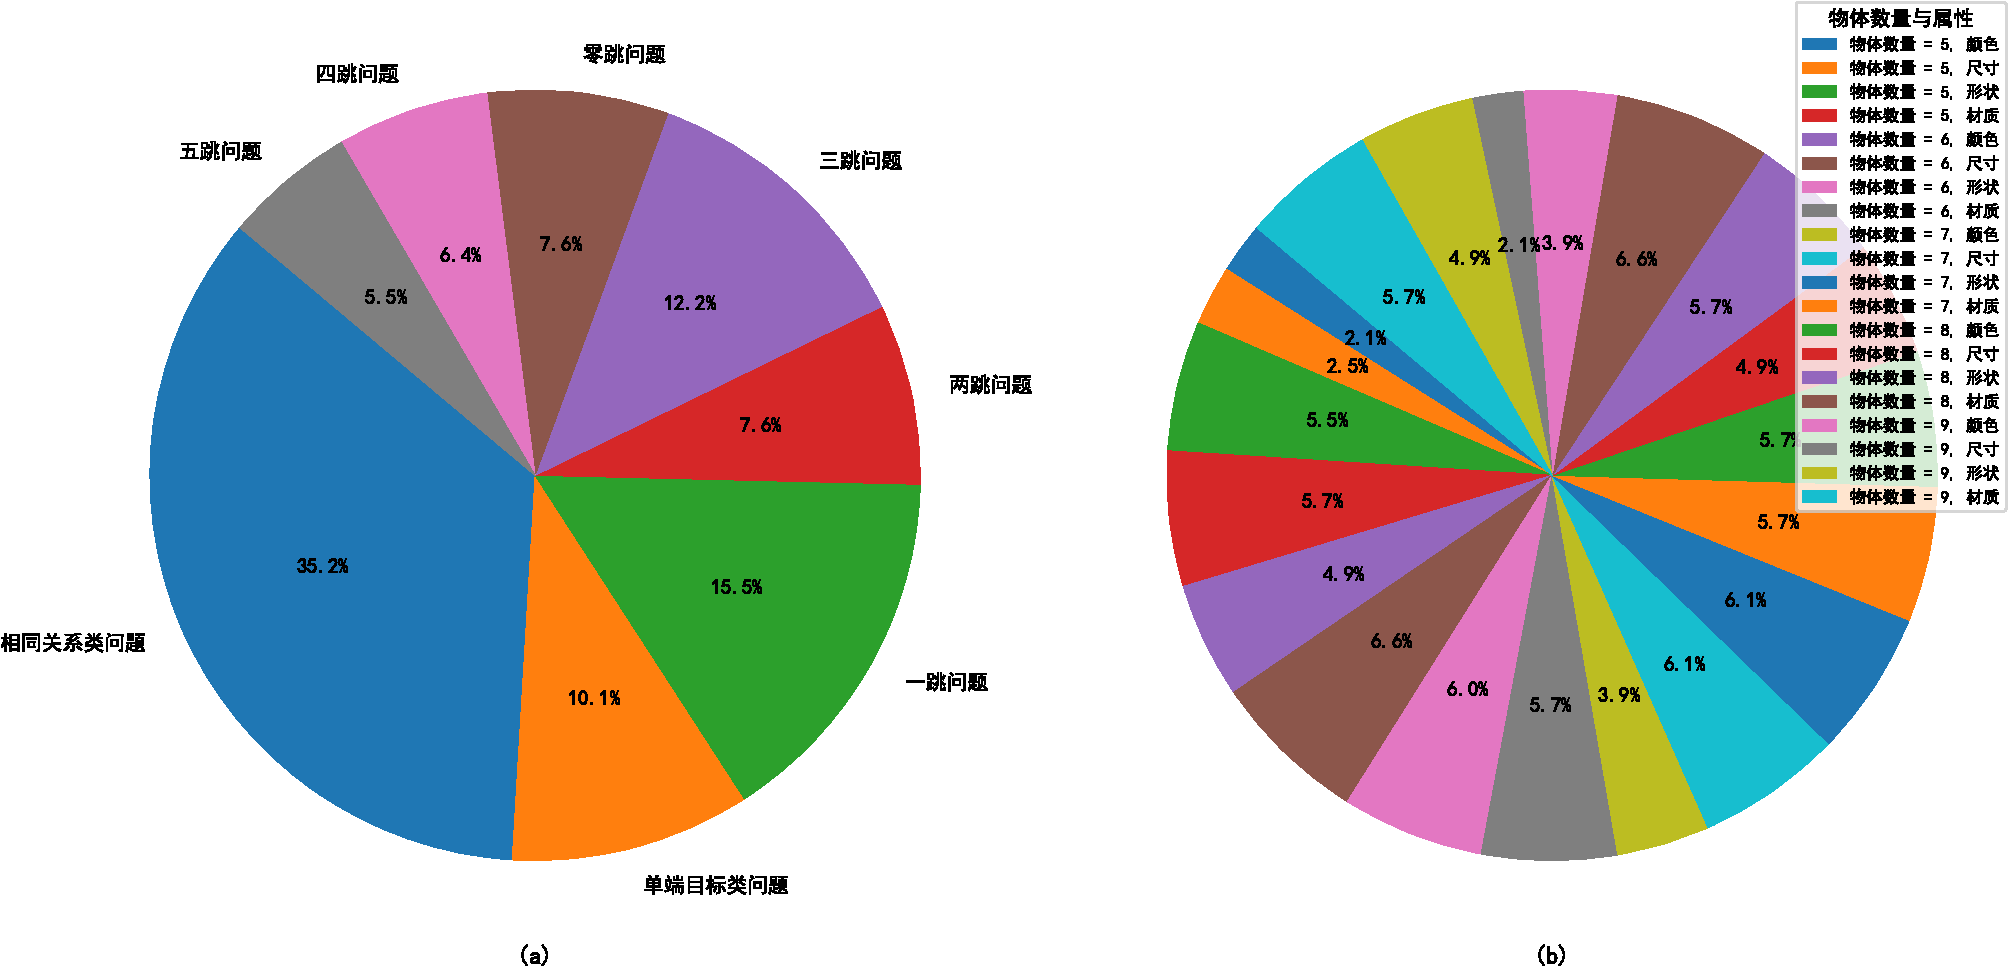
\includegraphics[scale=0.45]{figures/question_template_distribution-crop.pdf}
    \caption{(a)为问题模板分布,(b)查询属性在物体数量为5到9之间的分布}
    \label{fig:template_statistics}
\end{figure}
\subsection{合理性分析}
为了保证数据集的质量,采用双盲人工审核机制,邀请两名评审员各自独立对数据集进行评审。
在评审过程中,如果两名评审员同时判定该问题出现错误,那么将该问题剔除。
双盲评审的结果见表\ref{tab:kappa},其中展示了评审员1和评审员2分别与初始标注的一致性,以及两名评审员
之间的一致性。通过Fleiss's Kappa衡量的评审员间的一致性超过0.8,证明了数据集的可靠性。
\begin{table}[h]
    \centering
    \renewcommand{\arraystretch}{0.8}
    \begin{tabular}{lccc}
    \toprule
     & \makecell{答案是否正确} & \makecell{推理所需步数} & \makecell{问题是否可观察}\\
    \midrule
    初始标注与评审员1 & 81.2 & 84.4 & 89.6 \\
    初始标注与评审员2 & 84.2 & 85.6 & 85.4 \\
    评审员1与评审员2 & 80.1 & 83.8 & 86.9 \\
    \midrule
    平均值 & 81.8 & 84.6 & 87.3 \\
    \bottomrule
    \end{tabular}
    \caption{评审员1、2和初始标注之间的标注者间一致性}
    \label{tab:kappa}
\end{table}
本文通过记录2位评审员在POVQAD数据集上回答问题时的正确率、以及所需检索信息的次数、回答问题所需要的跳数,来对
数据集的难度进行判断,并于其它现有的VQA数据集进行比较。实验结果见表\ref{tab:human_performance},其中明显可以看出,POVQAD回答问题所需
的跳数,明显大于现有数据集VQAv2,另外POVQAD所需的检索信息的次数也更多一些,这些都证明了回答POVQAD数据集
所需的外部知识更多,考虑次数更多,数据集难度更大。另外,人类在本文
构造的POVQAD数据集上的准确率最低,进一步侧面印证了本文构造数据集的挑战性。
\begin{table}[h]
    \centering
    \renewcommand{\arraystretch}{0.8}
    \begin{tabular}{lccc}
    \toprule
     & \makecell{回答问题正确率} & \makecell{推理所需跳数} & \makecell{检索信息次数}\\
    \midrule
    POVQAD & 81.2 & 84.4 & 89.6 \\
    CLEVR & 84.2 & 85.6 & 85.4 \\
    GQAv2 & 80.1 & 83.8 & 86.9 \\
    \midrule
    平均值 & 81.8 & 84.6 & 87.3 \\
    \bottomrule
    \end{tabular}
    \caption{人类评审员在不同VQA数据集上回答问题的表现}
    \label{tab:human_performance}
\end{table}
\section{本章小结}
本章围绕POVQAD(Partial Observation VQA Dataset)数据集的设计与构建进行了系统介绍。
该数据集以CLEVR为基础,借鉴现实中信息不可完全观测的特点,引入了部分可见性、遮挡机制和复杂环境约束,
以更真实地模拟智能体在真实物理世界中所面临的推理挑战。

在设计目标方面,POVQAD明确提出要评估和提升模型在部分可见条件下的空间推理能力,
并通过引入区域属性与逻辑约束(使用ASP表示)为推理过程提供先验结构支持。在构建流程上,数据集经历了从环境生成、完整场景图生成、
部分场景图生成、问题与答案生成,再到图像渲染与表示转换的完整技术路径,确保数据在逻辑一致性、多样性与推理复杂性之间实现平衡。

此外,本章通过统计分析展示了问题模板、属性分布与答案空间的覆盖情况,证明了数据集在任务类型和解集结构上的均衡性。
质量评估与难度评估实验进一步佐证了数据集在标注一致性、问题合理性及推理复杂度等维度的高标准,
验证了POVQAD作为研究神经符号推理系统的重要基准集的实用价值和挑战性。

本章为后续神经符号VQA框架在复杂视觉问答任务中的实验与分析奠定了坚实的数据基础。